\subsection{Eulerovské a úplné bipartitní podgrafy}


\df Nechť $G = (V,E)$ je souvislý graf. {\it Spanning podgraf} (česky též \uv{napnutý} podgraf) grafu $G$ je graf obsahující všechny vrcholy a některé hrany $G$.

\medskip
Spanning podgraf ztotožníme s~jeho charakteristickým vektorem délky $|E|$. Sčítání spanning podgrafů nad $\GF(2)$ je realizováno symetrickou diferencí.

\begin{center}
	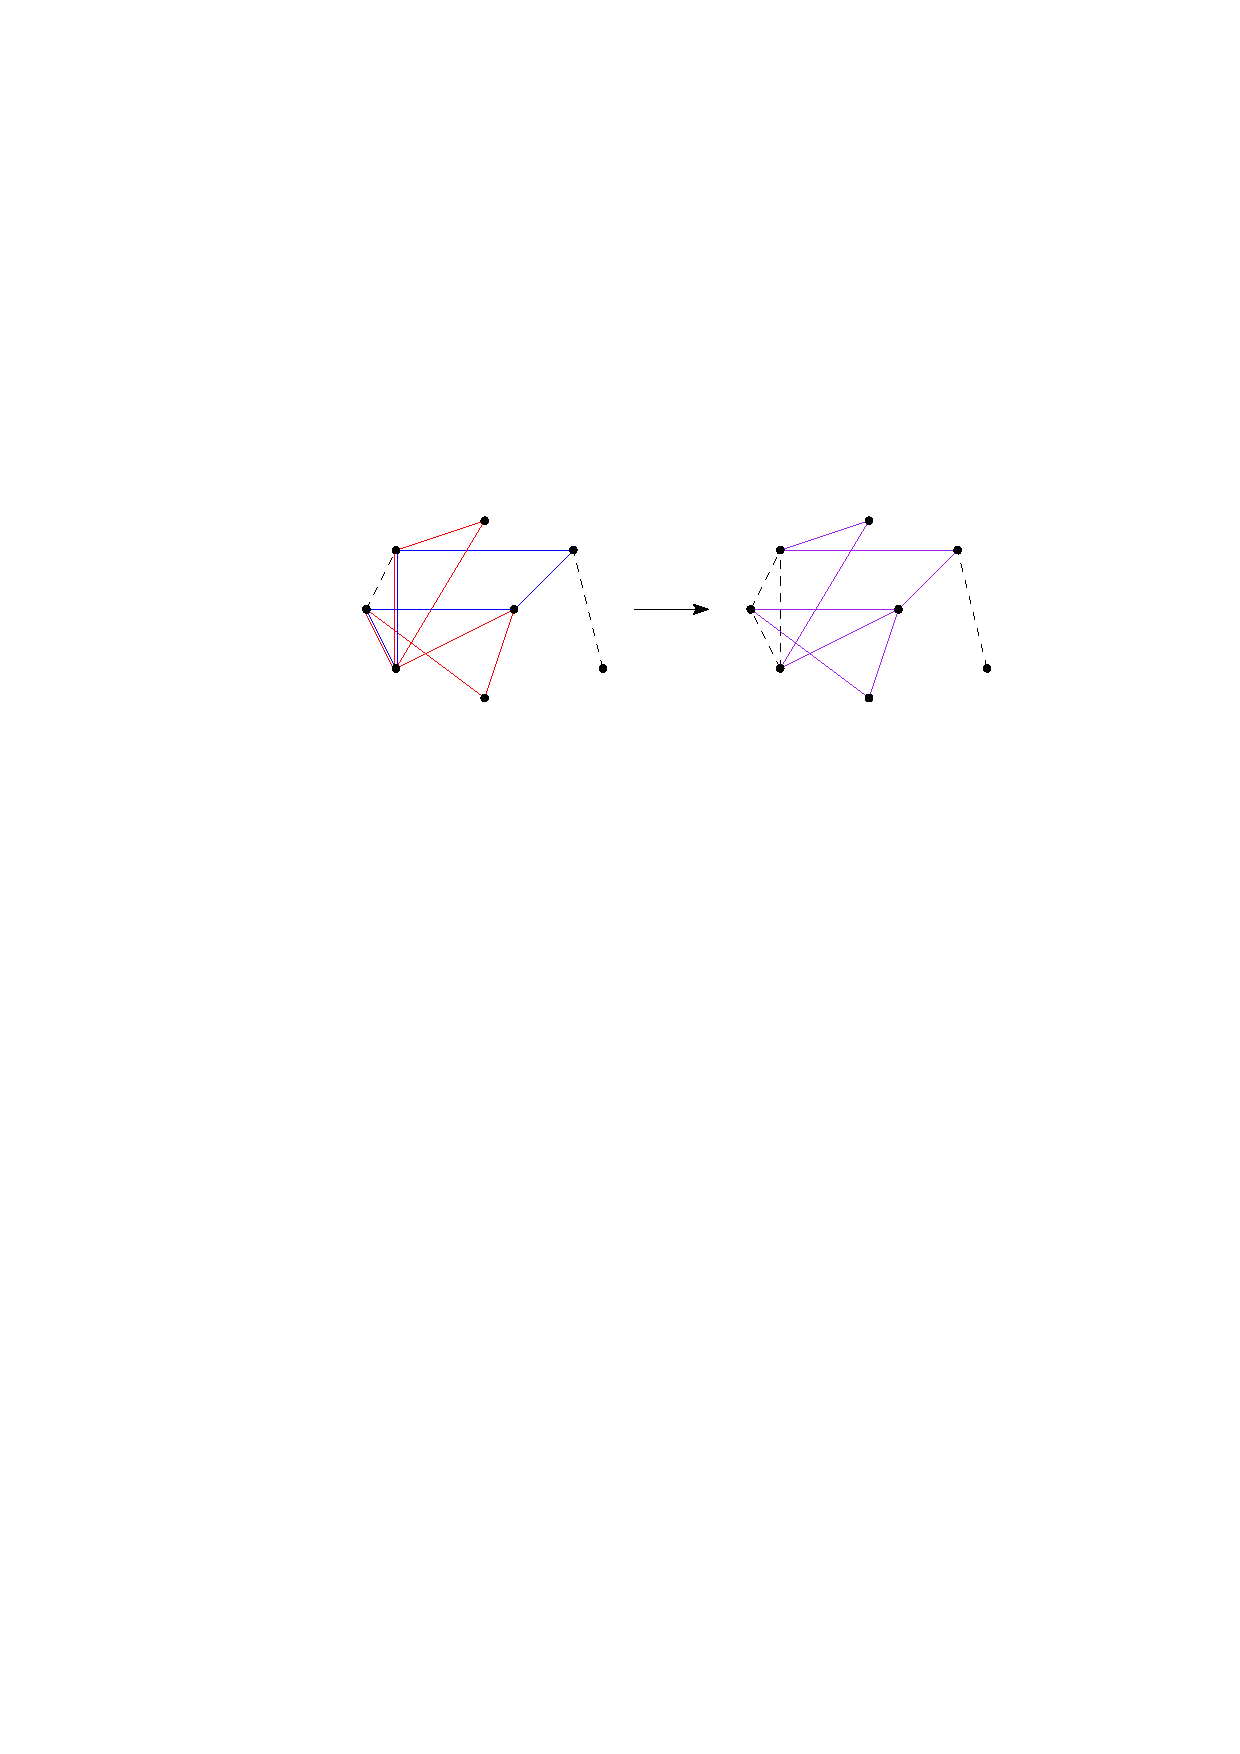
\includegraphics{symetricka_diference.pdf}
\end{center}

\tv Množina $V_G$ všech spanning podgrafů $G$ je vektorový prostor nad $\GF(2)$.

\df {\it Eulerovský spanning podgraf} grafu $G$ je takový spanning podgraf, který má všechny stupně sudé.

\medskip
Množinu všech eulerovských spanning podgrafů $G$ označme $\varepsilon_G$. Součtem dvou eulerovských podgrafů je zřejmě opět eulerovský podgraf, tedy $\varepsilon_G$ je podprostorem $V_G$.

\lm Platí $\dim \varepsilon_G = |E| - n + 1$, kde $n=|V|$.

\dk Nechť $T$ je libovolná kostra grafu $G$. Pro každou hranu $e\in E(G)\backslash E(T)$ existuje právě jedna elementární kružnice $K_e$ určená touto hranou. Množina
\begin{align}
K_T=\{ K_e\mid e \in E(G) \backslash E(T) \}
\end{align}
je lineárně nezávislá, neboť pro $e\in E(G)\backslash E(T)$ má kružnice $K_e$ jako jediná nenulovou $e$-tou souřadnici.

Pro $L\in\varepsilon_G$ položme
\begin{align}
	L'=\hspace{-10pt}\sum_{e\in E(L)\backslash E(T)}\hspace{-10pt}K_e.
\end{align}
Graf $L+L'$ neobsahuje žádné hrany mimo kostru a současně je součtem eulerovských grafů, tedy je nutně eulerovský. Jediným eulerovským podgrafem kostry je $0$, což znamená, že $L+L'=0$ a $L=L'$. Tedy $K_T$ tvoří bázi $\varepsilon_G$ a platí $\dim \varepsilon_G = |K_t|=|E| - n + 1$.\qed

\df {\it Úplný bipartitní spanning podgraf} grafu $G$ je řez v~$G$.

\begin{center}
	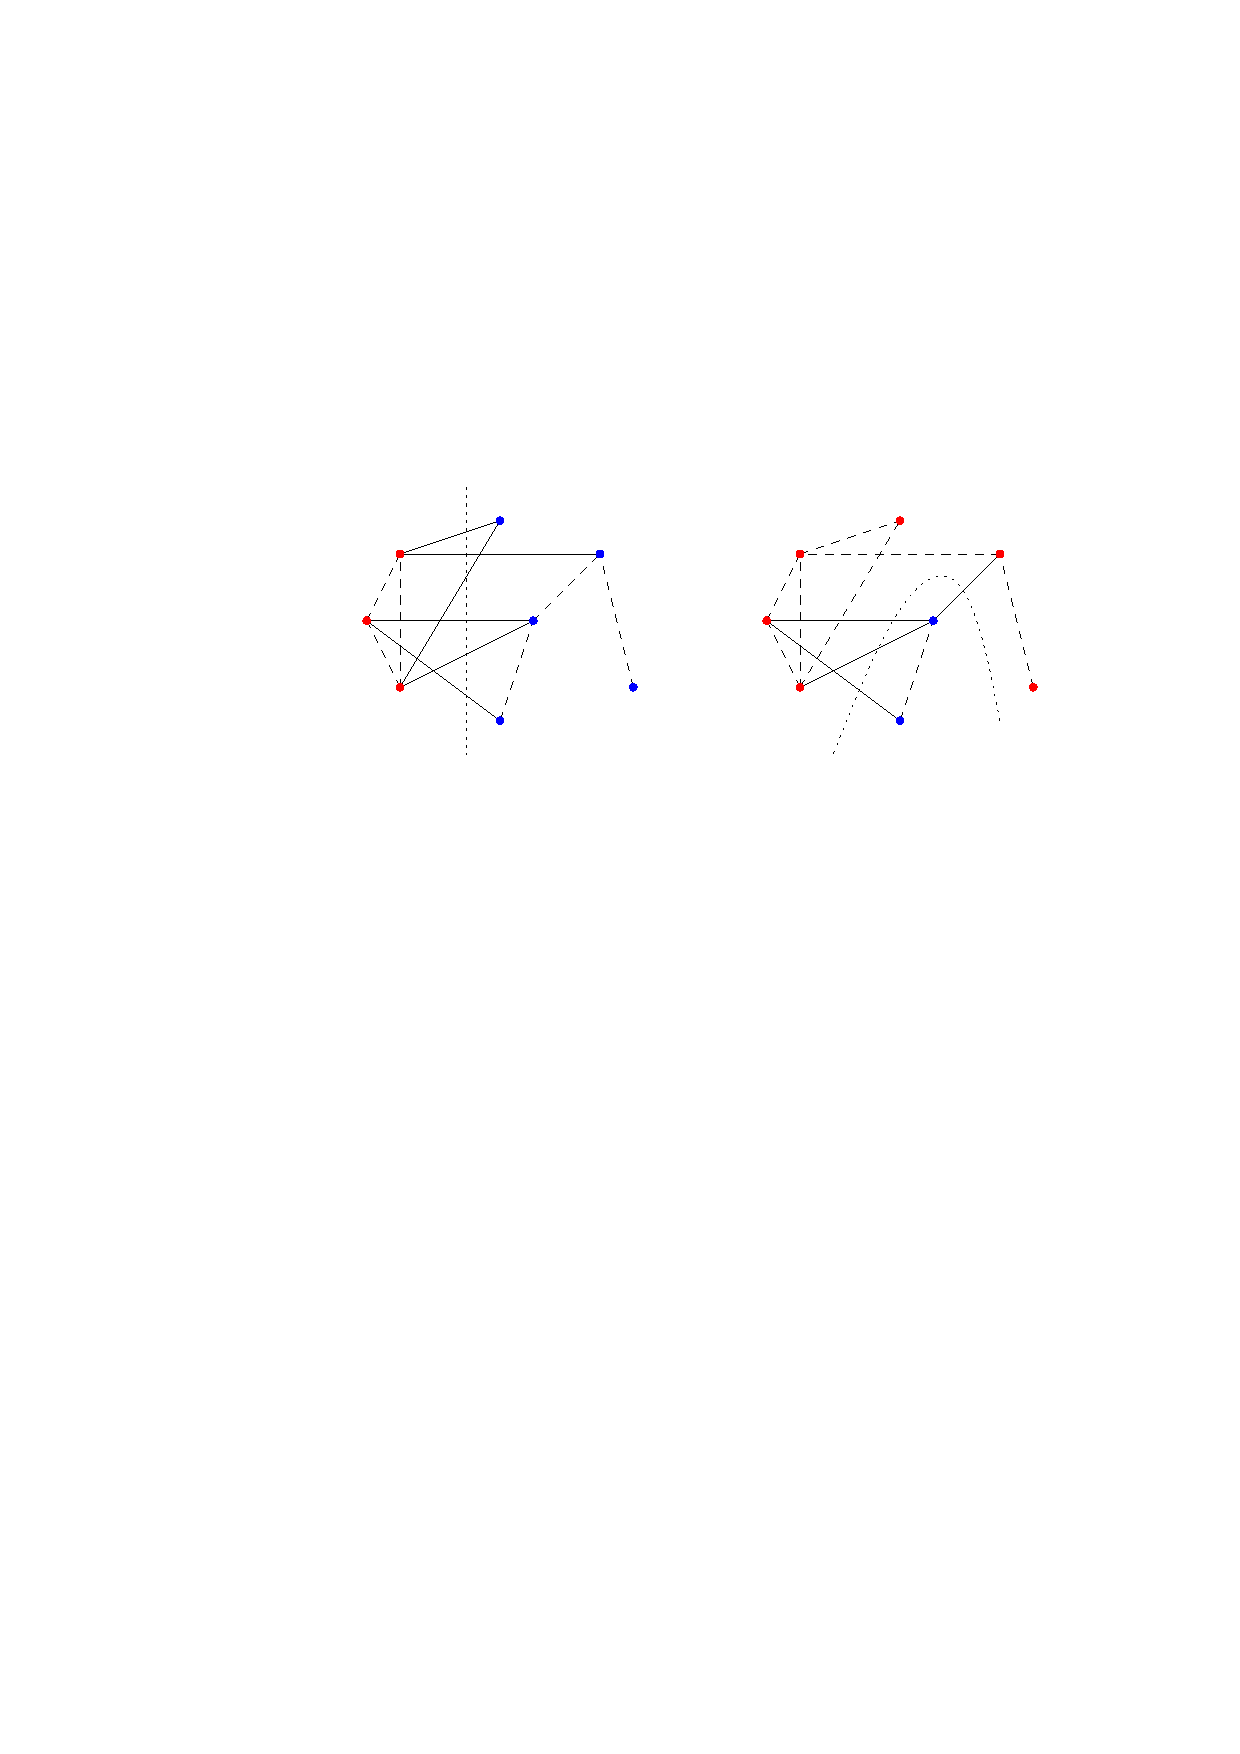
\includegraphics{uplny_bipartitni_spanning.pdf}
\end{center}

\medskip
Množinu všech úplných bipartitních spanning podgrafů $G$ označme $\beta_G$. 

\lm Množina $\beta_G$ tvoří podprostor $V_G$, jehož množinou generátorů jsou všechny hvězdy v~$G$. Platí $\dim\beta_G=n-1$.

\dk Každý úplný bipartitní spanning podgraf je součtem hvězd ze všech vrcholů jedné z~jeho partit. K~nahlédnutí, že součet dvou úplných bipartitních spanning podgrafů je opět úplný bipartitní spanning podgraf, stačí oba grafy rozepsat na součet hvězd.

Všimněme si, že součet hvězd ze všech vrcholů $G$ je $0$, ovšem libovolných $n-1$ hvězd už tvoří lineárně nezávislou množinu. Netriviální lineární kombinace $n-1$ hvězd s~koeficienty v~$\GF(2)$ je totiž jen součet několika (aspoň jedné a nejvýše $n-1$) z~nich. Ten není nikdy nulový, neboť v~$G$ existuje hrana, pro niž se v~lineární kombinaci vyskytuje hvězda z~právě jednoho z~jejích koncových vrcholů. Tedy $\dim\beta_G=n-1$.

\vt Platí $\varepsilon_G^\bot = \beta_G$.

\dk Buď $H \in \varepsilon_G$, $u \in V(G)$ a $S_u$ hvězda z~vrcholu $u$. Protože
\begin{align*}
\sk{H,S_u}= \deg_H u\text{ mod }2=0,
\end{align*}
platí $\sk{H,B} = 0$ pro všechna $B\in\beta_G$, a tedy $H \in \beta_G^\bot$, což dává inkluzi $\varepsilon_G \subseteq \beta_G^\bot$.

Naopak, každý spanning podgraf $H$, pro který je $\sk{H,S_u} = 0$, má nutně všechny stupně sudé, a je tedy eulerovský. Proto je rovněž $\beta_G^\bot \subseteq \varepsilon_G$ a věta je dokázána.\qed

\vt Je-li $M$ podprostorem $\GF(2)^n$, pak $(1,\dots,1) \in M + M^\bot$.

\dk Je-li $\dim(M \cap M^\bot) = 0$, pak $\dim(M + M^\bot) = n$, tedy zřejmě platí $(1,\dots,1)\in M$. Jestliže $\dim(M \cap M^\bot) > 0$, pak existuje $x=(x_1,\dots,x_n)\in M\cap M^\bot$, $x\neq0$. Dále
\begin{align}
\sk{x,(1,\dots,1)}=\sum_{i=1}^n x_i=\sum_{i=1}^n x_i^2=\sk{x,x}=0,
\end{align}
tedy $(1,\dots,1)\bot x$ a nutně platí $(1,\dots,1)\in M + M^\bot$.\qed

\dsl Každý souvislý graf lze zapsat jako symetrickou diferenci eulerovského podgrafu a hranového řezu.

\dk V~prostoru $V_G$ je podle předchozí věty $G=(1,\dots,1)\in\varepsilon_G+\beta_G$, tedy existují grafy $H\in\varepsilon_G$ a $B\in\beta_G$ takové, že $H+B=G$.\qed